%% How to compile by hand, not in package: 
% R --vanilla
% library(knitr)
% knit("intro.Rnw")
%knit2pdf("intro.Rnw")
%do not ever type .tex!!!!

%after creating intro.pdf:
%comment out the first code chunk (options)
%delete .bbl and .blg files
%copy the pdf to inst/doc
%build
%R CMD check --as-cran
%ship

\documentclass[11pt]{article}\usepackage[]{graphicx}\usepackage[]{color}
% maxwidth is the original width if it is less than linewidth
% otherwise use linewidth (to make sure the graphics do not exceed the margin)
\makeatletter
\def\maxwidth{ %
  \ifdim\Gin@nat@width>\linewidth
    \linewidth
  \else
    \Gin@nat@width
  \fi
}
\makeatother

\definecolor{fgcolor}{rgb}{0.345, 0.345, 0.345}
\newcommand{\hlnum}[1]{\textcolor[rgb]{0.686,0.059,0.569}{#1}}%
\newcommand{\hlstr}[1]{\textcolor[rgb]{0.192,0.494,0.8}{#1}}%
\newcommand{\hlcom}[1]{\textcolor[rgb]{0.678,0.584,0.686}{\textit{#1}}}%
\newcommand{\hlopt}[1]{\textcolor[rgb]{0,0,0}{#1}}%
\newcommand{\hlstd}[1]{\textcolor[rgb]{0.345,0.345,0.345}{#1}}%
\newcommand{\hlkwa}[1]{\textcolor[rgb]{0.161,0.373,0.58}{\textbf{#1}}}%
\newcommand{\hlkwb}[1]{\textcolor[rgb]{0.69,0.353,0.396}{#1}}%
\newcommand{\hlkwc}[1]{\textcolor[rgb]{0.333,0.667,0.333}{#1}}%
\newcommand{\hlkwd}[1]{\textcolor[rgb]{0.737,0.353,0.396}{\textbf{#1}}}%
\let\hlipl\hlkwb

\usepackage{framed}
\makeatletter
\newenvironment{kframe}{%
 \def\at@end@of@kframe{}%
 \ifinner\ifhmode%
  \def\at@end@of@kframe{\end{minipage}}%
  \begin{minipage}{\columnwidth}%
 \fi\fi%
 \def\FrameCommand##1{\hskip\@totalleftmargin \hskip-\fboxsep
 \colorbox{shadecolor}{##1}\hskip-\fboxsep
     % There is no \\@totalrightmargin, so:
     \hskip-\linewidth \hskip-\@totalleftmargin \hskip\columnwidth}%
 \MakeFramed {\advance\hsize-\width
   \@totalleftmargin\z@ \linewidth\hsize
   \@setminipage}}%
 {\par\unskip\endMakeFramed%
 \at@end@of@kframe}
\makeatother

\definecolor{shadecolor}{rgb}{.97, .97, .97}
\definecolor{messagecolor}{rgb}{0, 0, 0}
\definecolor{warningcolor}{rgb}{1, 0, 1}
\definecolor{errorcolor}{rgb}{1, 0, 0}
\newenvironment{knitrout}{}{} % an empty environment to be redefined in TeX

\usepackage{alltt}

%\VignetteEngine{knitr::knitr}
%\VignetteIndexEntry{Using mcmcse}
%\VignettePackage{mcmcse}
%\VignetteKeywords{Markov chain Monte Carlo, batch means}

\usepackage{amsmath}
\usepackage[sort,longnamesfirst]{natbib}
\usepackage{verbatim}   % useful for program listings
\usepackage{amsfonts, framed}
\usepackage[small,compact]{titlesec} 
\title{An Introduction to Estimating Monte Carlo Standard Errors with R Package \texttt{mcmcse} }
\author{Dootika Vats}
\IfFileExists{upquote.sty}{\usepackage{upquote}}{}
\begin{document}


\maketitle
\setlength\parindent{0pt}
\tableofcontents

\break
\section{Introduction}
The R package \texttt{mcmcse} provides estimates of Monte Carlo standard errors for Markov chain Monte Carlo (MCMC) when estimating means or quantiles of functions of the MCMC output. In addition to MCMC output, the package can be used for time series and other correlated processes. 

The package is predominantly useful after MCMC output has been obtained by the user. In addition to estimating the Monte Carlo standard errors, the package also provides univariate and multivariate estimates of effective sample size and tools to determine whether enough Monte Carlo samples have been obtained. There are also some graphical tools to ascertain the behavior of the Monte Carlo estimates.


%<<noname,echo=FALSE>>=
%library(knitr)
%opts_chunk$set(comment = NA,background='white')
%opts_knit$set(out.format = "latex")
%knit_theme$set("seashell")
%@

\bigskip
\section{An MCMC Example}

To illustrate the use of our package, we present the following simple multivariate AR(1) process. The process is defined for $t = 1, 2, 3, \dots$ as,
\[y_t = w + A y_{t-1} + \epsilon_t, \]

where $w$ is a constant vector in $\mathbb{R}^p$, $y_t \in \mathbb{R}^p$, $A$ is a $p \times p$ matrix and $\epsilon_t \sim N_p(0, C)$. In our example, we let $A$ and $C$ be diagonal matrices. The invariant distrbution for this process is $F = N_p(0, V)$ where $V$ is a function of $A$ and $C$. 

The function \texttt{mAr.sim} in package \texttt{mAr} draws samples from the above model. We let $p = 3$.

\begin{knitrout}
\definecolor{shadecolor}{rgb}{0.969, 0.969, 0.969}\color{fgcolor}\begin{kframe}
\begin{alltt}
\hlkwd{library}\hlstd{(mAr)}
\end{alltt}


{\ttfamily\noindent\itshape\color{messagecolor}{\#\# Loading required package: MASS}}\begin{alltt}
\hlstd{p} \hlkwb{<-} \hlnum{3}
\hlstd{A} \hlkwb{<-} \hlkwd{diag}\hlstd{(}\hlkwd{c}\hlstd{(}\hlnum{.1}\hlstd{,} \hlnum{.5}\hlstd{,} \hlnum{.8}\hlstd{))}
\hlstd{C} \hlkwb{<-} \hlkwd{diag}\hlstd{(}\hlkwd{rep}\hlstd{(}\hlnum{2}\hlstd{,} \hlnum{3}\hlstd{))}

\hlcom{# Monte Carlo sample size is N}
\hlstd{N} \hlkwb{<-} \hlnum{1e5}
\hlkwd{set.seed}\hlstd{(}\hlnum{100}\hlstd{)}
\hlstd{chain} \hlkwb{<-} \hlkwd{mAr.sim}\hlstd{(}\hlkwc{w} \hlstd{=} \hlkwd{rep}\hlstd{(}\hlnum{2}\hlstd{,p),} \hlkwc{A} \hlstd{= A,} \hlkwc{C} \hlstd{= C,} \hlkwc{N} \hlstd{= N)}
\end{alltt}
\end{kframe}
\end{knitrout}

For using the \texttt{mcmcse} package the rows of the MCMC output should store each iteration of the algorithm and so the output should have $n$ rows and $p$ columns. We will denote each row $i$ of the output as $y_i = (y^{(1)}_i, y^{(2)}_i, y^{(3)}_i)$.

\begin{knitrout}
\definecolor{shadecolor}{rgb}{0.969, 0.969, 0.969}\color{fgcolor}\begin{kframe}
\begin{alltt}
\hlcom{#Rows has observations (samples) and each comlumn is a component. }
\hlkwd{head}\hlstd{(chain)}
\end{alltt}
\begin{verbatim}
##           Y1       Y2        Y3
## 1 -0.3101768 3.967189  8.421232
## 2  5.2384324 6.391334 10.407224
## 3  2.5886888 6.497850 11.156644
## 4  3.8339966 4.992644 12.447253
## 5 -0.2396186 4.900606 13.565273
## 6  2.2108764 5.144180 13.927434
\end{verbatim}
\end{kframe}
\end{knitrout}

\bigskip
This vignette will discuss estimating two sets of features of interest of $F$.
\begin{itemize}
	\item $\text{E}_F y$: For estimating $\mu = \text{E}_Fy$, the estimator is the Monte Carlo sample mean
\[ \mu_n = \dfrac{1}{n} \displaystyle \sum_{t=1}^{n} y_t.\]

In \texttt{R}, $\mu_n$ is obtained using the usual \texttt{colMeans} function. If $p = 1$, then use \texttt{mean} instead of \texttt{colMeans}.

\begin{knitrout}
\definecolor{shadecolor}{rgb}{0.969, 0.969, 0.969}\color{fgcolor}\begin{kframe}
\begin{alltt}
 \hlkwd{colMeans}\hlstd{(chain)}
\end{alltt}
\begin{verbatim}
##        Y1        Y2        Y3 
##  2.225577  4.012947 10.007805
\end{verbatim}
\end{kframe}
\end{knitrout}

	\item $\text{E}_F \left(y^{(1)2} + y^{(2)2} + y^{(3)2} \right)$: When interested in estimating the sum of the second moments of each component of $y$,  define the function $g: \mathbb{R}^3 \to \mathbb{R}$ as $g((x_1,x_2,x_3)) = x_1^2 + x_2^2 + x_3^2$. This is defined in \texttt{R} by creating a function that implements the function $g$, row-wise.

\begin{knitrout}
\definecolor{shadecolor}{rgb}{0.969, 0.969, 0.969}\color{fgcolor}\begin{kframe}
\begin{alltt}
\hlstd{g} \hlkwb{<-} \hlkwa{function}\hlstd{(}\hlkwc{x}\hlstd{)}
\hlstd{\{}
        \hlkwd{return}\hlstd{(}\hlkwd{sum}\hlstd{(x}\hlopt{^}\hlnum{2}\hlstd{))}
\hlstd{\}}
\end{alltt}
\end{kframe}
\end{knitrout}

The Monte Carlo estimator for $g$ is 
\[ \mu_{g,n} = \dfrac{1}{n} \displaystyle \sum_{t=1}^{n} g(y_t),\]

\begin{knitrout}
\definecolor{shadecolor}{rgb}{0.969, 0.969, 0.969}\color{fgcolor}\begin{kframe}
\begin{alltt}
\hlcom{# Apply the function g to each row}
\hlstd{gofy} \hlkwb{<-} \hlkwd{apply}\hlstd{(chain,} \hlnum{1}\hlstd{, g)}

\hlcom{# Monte Carlo estimate}
\hlkwd{mean}\hlstd{(gofy)}
\end{alltt}
\begin{verbatim}
## [1] 131.4661
\end{verbatim}
\end{kframe}
\end{knitrout}
\end{itemize}

Thus, to obtain Monte Carlo estimates from MCMC output, the base package is sufficient (generally). However, Monte Carlo estimates must be reported with Monte Carlo standard error. That is, if the following central limit theorems hold
\begin{equation}
\label{eq:clt}
\sqrt{n}(\mu_n - \mu) \overset{d}{\to} N_p(0, \Sigma)\,,
\end{equation}
and

\begin{equation}
\label{eq:g_clt}
\sqrt{n}(\mu_{g,n} - \mu) \overset{d}{\to} N_p(0, \Sigma_g)\,,
\end{equation}

then estimates of $\Sigma$ and $\Sigma_g$ must be reported, directly or indirectly. Since the samples obtained are correlated, these quantities require more sophisticated tools than usual sample estimators.
(Note that a Markov chain CLT is not always guaranteed to hold. In fact, it depends on the rate of convergence of the Markov chain. Most of the functions in this package assume that a Markov chain CLT holds. Such an assumption is also made when using many of the convergence diagnostics).

\section{Estimating Monte Carlo Standard Error}
In this package, the functions \texttt{mcse}, \texttt{mcse.mat}, \texttt{mcse.multi}, and \texttt{mcse.initseq} estimate the Monte Carlo standard error of $\mu_n$ (or $\mu_{g,n}$).
\begin{itemize}
\item \texttt{mcse}: consistent estimates of $\sqrt{\Sigma/n}$ (standard error) when $\Sigma$ is $1 \times 1$. 
\item \texttt{mcse.mat}: consistent estimates of the square root of the  diagonals of $\Sigma/n$.
\item \texttt{mcse.multi}: consistent estimates of $\Sigma$.
\item \texttt{mcse.initseq}: asymptotically conservative estimates of $\Sigma$ using initial sequence estimators.
\end{itemize}

Using the \texttt{mcmcse} package we can estimate $\Sigma$ in \eqref{eq:clt} with the \texttt{mcse.multi} and \texttt{mcse.initseq} function. 

\begin{knitrout}
\definecolor{shadecolor}{rgb}{0.969, 0.969, 0.969}\color{fgcolor}\begin{kframe}
\begin{alltt}
\hlkwd{library}\hlstd{(mcmcse)}
\end{alltt}


{\ttfamily\noindent\itshape\color{messagecolor}{\#\# mcmcse: Monte Carlo Standard Errors for MCMC\\\#\# Version 1.3-4 created on 2019-12-21.\\\#\# copyright (c) 2012, James M. Flegal, University of California, Riverside\\\#\#\ \ \ \ \ \ \ \ \ \ \ \ \ \ \ \ \ \ \ \  John Hughes, University of Colorado, Denver\\\#\#\ \ \ \ \ \ \ \ \ \ \ \ \ \ \ \ \ \ \ \  Dootika Vats, University of Warwick\\\#\#\ \ \ \ \ \ \ \ \ \ \ \ \ \ \ \ \ \ \ \  Ning Dai, University of Minnesota\\\#\#\ \ For citation information, type citation("{}mcmcse"{}).\\\#\#\ \ Type help("{}mcmcse-package"{}) to get started.}}\begin{alltt}
\hlcom{# Batch means estimator}
\hlstd{mcerror_bm} \hlkwb{<-} \hlkwd{mcse.multi}\hlstd{(}\hlkwc{x} \hlstd{= chain,} \hlkwc{method} \hlstd{=}  \hlstr{"bm"}\hlstd{,} \hlkwc{r} \hlstd{=} \hlnum{1}\hlstd{,}
        \hlkwc{size} \hlstd{=} \hlkwa{NULL}\hlstd{,} \hlkwc{g} \hlstd{=} \hlkwa{NULL}\hlstd{,} \hlkwc{adjust} \hlstd{=} \hlnum{TRUE}\hlstd{,} \hlkwc{blather} \hlstd{=} \hlnum{TRUE}\hlstd{)}

\hlcom{# Overlapping batch means estimator}
\hlstd{mcerror_bm} \hlkwb{<-} \hlkwd{mcse.multi}\hlstd{(}\hlkwc{x} \hlstd{= chain,} \hlkwc{method} \hlstd{=}  \hlstr{"obm"}\hlstd{,} \hlkwc{r} \hlstd{=} \hlnum{1}\hlstd{,}
        \hlkwc{size} \hlstd{=} \hlkwa{NULL}\hlstd{,} \hlkwc{g} \hlstd{=} \hlkwa{NULL}\hlstd{,} \hlkwc{adjust} \hlstd{=} \hlnum{TRUE}\hlstd{,} \hlkwc{blather} \hlstd{=} \hlnum{TRUE}\hlstd{)}

\hlcom{# Spectral variance estimator with Bartlett window}
\hlstd{mcerror_bart} \hlkwb{<-} \hlkwd{mcse.multi}\hlstd{(}\hlkwc{x} \hlstd{= chain,} \hlkwc{method} \hlstd{=}  \hlstr{"bartlett"}\hlstd{,} \hlkwc{r} \hlstd{=} \hlnum{1}\hlstd{,}
        \hlkwc{size} \hlstd{=} \hlkwa{NULL}\hlstd{,} \hlkwc{g} \hlstd{=} \hlkwa{NULL}\hlstd{,} \hlkwc{adjust} \hlstd{=} \hlnum{TRUE}\hlstd{,} \hlkwc{blather} \hlstd{=} \hlnum{TRUE}\hlstd{)}

\hlcom{# Spectral variance estimator with Tukey window}
\hlstd{mcerror_tuk} \hlkwb{<-} \hlkwd{mcse.multi}\hlstd{(}\hlkwc{x} \hlstd{= chain,} \hlkwc{method} \hlstd{=}  \hlstr{"tukey"}\hlstd{,} \hlkwc{r} \hlstd{=} \hlnum{1}\hlstd{,}
        \hlkwc{size} \hlstd{=} \hlkwa{NULL}\hlstd{,} \hlkwc{g} \hlstd{=} \hlkwa{NULL}\hlstd{,} \hlkwc{adjust} \hlstd{=} \hlnum{TRUE}\hlstd{,} \hlkwc{blather} \hlstd{=} \hlnum{TRUE}\hlstd{)}

\hlcom{# Initial sequence estimator, unadjusted}
\hlstd{mcerror_is} \hlkwb{<-} \hlkwd{mcse.initseq}\hlstd{(}\hlkwc{x} \hlstd{= chain,} \hlkwc{g} \hlstd{=} \hlkwa{NULL}\hlstd{,}
                           \hlkwc{adjust} \hlstd{=} \hlnum{FALSE}\hlstd{,} \hlkwc{blather} \hlstd{=} \hlnum{TRUE}\hlstd{)}

\hlcom{# Initial sequence estimator, adjusted}
\hlstd{mcerror_isadj} \hlkwb{<-} \hlkwd{mcse.initseq}\hlstd{(}\hlkwc{x} \hlstd{= chain,} \hlkwc{g} \hlstd{=} \hlkwa{NULL}\hlstd{,}
                              \hlkwc{adjust} \hlstd{=} \hlnum{TRUE}\hlstd{,} \hlkwc{blather} \hlstd{=} \hlnum{TRUE}\hlstd{)}
\end{alltt}
\end{kframe}
\end{knitrout}

\begin{itemize}
	\item \texttt{x} takes the $n \times p$ MCMC data. \texttt{x} can take only numeric entries in the form of a matrix or data frame. The rows of \texttt{x} are the iterations of the MCMC.

	\item \texttt{method = bm, obm, bartlett, tukey} calculates the estimate using the batch means method and spectral variance methods with the modified-Bartlett and Tukey-Hanning windows.
	
	\item \texttt{r} is the lugsail parameter that indicates how much to "lift" the lag window (this also  applies to \texttt{bm} and \texttt{obm}). Higher values will increasingly remove underestimation of $\Sigma$ but may yield more variable estimators. Values more than 5 are not advised and negative values are not allowed. Reasonable choices are $r = 1, 2, 3$, where $r = 3$ yields the lugsail estimator, $r = 2$ is the flat-top estimator, and $r = 1$ is the vanilla estimator. 

	\item \texttt{size} is the batch size for the \texttt{bm} method and the truncation point for \texttt{tukey} and \texttt{bartlett} methods. Default batch size is calulcated using the exported \texttt{batchSize} function. Other accepted values are \texttt{size = sqroot}, which sets the size as $\lfloor \sqrt{n} \rfloor$ and \texttt{size = cuberoot} which sets it at $\lfloor n^{1/3} \rfloor$. An integer value of \texttt{size} less than $n$ is also valid as long as $n/\texttt{size} > 1$.
	
For reference on \texttt{bm} (batch means estimators) see \cite{jones2006fixed} and \cite{vats:fleg:jones:2017b}.

For reference on \texttt{bartlett} and \texttt{tukey} (spectral variance estimators)see \cite{flegal2010batch} and \cite{vats2015strong}.

For reference on lugsail estimation see \cite{liu:fleg:2018} and \cite{vats:fleg:2018}.

	\item \texttt{g} is a function that is applied to each row of \texttt{x} and represents the features of interest of the process. Since here we are interested in only means, \texttt{g} is \texttt{NULL}. \texttt{g} will be explained in later examples.
	
	\item \texttt{adjust} is a logical argument indicating whether the resulting matrix should be adjusted in order to retain positive-definiteness. By default this is set to be \texttt{TRUE}.
	
	\item \texttt{blather} when TRUE outputs under the hood information about the estimation process. The default is set to \texttt{FALSE} since most users should be interested in only \texttt{cov} and \texttt{est}.
	
For reference on \texttt{mcse.initseq} (initial sequence estimators) see \cite{dai2017multivariate}.
\end{itemize}

\texttt{mcse.multi} and \texttt{mcse.initseq} return a list with multiple components. When \texttt{blather = FALSE} \texttt{cov} stores the estimate of $\Sigma$ obtained using the method chosen, \texttt{est} stores the estimate of the mean of $g$ applied on the Markov chain. When \texttt{blather = TRUE} the following are returned in addition to the above two: \texttt{nsim}  stores the arguments used to calculate $\Sigma$.  \texttt{size} which indicates the size of batches/truncation, \texttt{method} used. \texttt{mcse.initseq} also returns \texttt{cov.adj}, and whether an adjusted estimator was used (\texttt{adjust}).

\begin{knitrout}
\definecolor{shadecolor}{rgb}{0.969, 0.969, 0.969}\color{fgcolor}\begin{kframe}
\begin{alltt}
\hlstd{mcerror_bm}\hlopt{$}\hlstd{cov}
\end{alltt}
\begin{verbatim}
##            [,1]        [,2]        [,3]
## [1,]  2.6008515 -0.18030089  0.17474396
## [2,] -0.1803009  7.84219221  0.07412673
## [3,]  0.1747440  0.07412673 47.87634711
\end{verbatim}
\begin{alltt}
\hlstd{mcerror_bart}\hlopt{$}\hlstd{cov}
\end{alltt}
\begin{verbatim}
##            [,1]       [,2]       [,3]
## [1,]  2.6026895 -0.1815027  0.1688387
## [2,] -0.1815027  7.8446983  0.0830542
## [3,]  0.1688387  0.0830542 47.9195206
\end{verbatim}
\begin{alltt}
\hlstd{mcerror_tuk}\hlopt{$}\hlstd{cov}
\end{alltt}
\begin{verbatim}
##            [,1]         [,2]         [,3]
## [1,]  2.6218068 -0.197829185  0.167027884
## [2,] -0.1978292  7.907577433 -0.006610122
## [3,]  0.1670279 -0.006610122 49.188066347
\end{verbatim}
\begin{alltt}
\hlstd{mcerror_is}\hlopt{$}\hlstd{cov}
\end{alltt}
\begin{verbatim}
##            [,1]        [,2]        [,3]
## [1,]  2.5029696 -0.10902926  0.11007175
## [2,] -0.1090293  8.18913933  0.02202062
## [3,]  0.1100717  0.02202062 50.96199582
\end{verbatim}
\begin{alltt}
\hlstd{mcerror_isadj}\hlopt{$}\hlstd{cov.adj}
\end{alltt}
\begin{verbatim}
##             [,1]         [,2]         [,3]
## [1,]  2.58127094 -0.060426547  0.083477237
## [2,] -0.06042655  8.242248961 -0.002410464
## [3,]  0.08347724 -0.002410464 51.034334815
\end{verbatim}
\begin{alltt}
\hlkwd{rbind}\hlstd{(mcerror_bm}\hlopt{$}\hlstd{est, mcerror_bart}\hlopt{$}\hlstd{est, mcerror_tuk}\hlopt{$}\hlstd{est,}
      \hlstd{mcerror_is}\hlopt{$}\hlstd{est, mcerror_isadj}\hlopt{$}\hlstd{est)}
\end{alltt}
\begin{verbatim}
##            Y1       Y2       Y3
## [1,] 2.225577 4.012947 10.00781
## [2,] 2.225577 4.012947 10.00781
## [3,] 2.225577 4.012947 10.00781
## [4,] 2.225577 4.012947 10.00781
## [5,] 2.225577 4.012947 10.00781
\end{verbatim}
\end{kframe}
\end{knitrout}



\textbf{Note: } The Monte Carlo estimates of $\mu$ are not affected by the choice of the method.

\bigskip
\textbf{Note: } for consistent estimation, the batch means estimators are significantly faster to calculate than the spectral variance estimators. The user is advised to use the default \texttt{method = ``bm''} for large input matrices.

\bigskip
\textbf{Note: }\texttt{cov} returns an estimate of $\Sigma$ and not $\Sigma/n$. 

\bigskip
If the diagonals of $\Sigma$ are $\sigma_{ii}^2$, the function \texttt{mcse} and \texttt{mcse.mat} returns $\sigma_{ii}/\sqrt{n}$. \texttt{mcse} does it for one component and \texttt{mcse.mat} does it for all diagonals.

\begin{knitrout}
\definecolor{shadecolor}{rgb}{0.969, 0.969, 0.969}\color{fgcolor}\begin{kframe}
\begin{alltt}
\hlkwd{mcse}\hlstd{(}\hlkwc{x} \hlstd{= chain[,}\hlnum{1}\hlstd{],} \hlkwc{method} \hlstd{=} \hlstr{"bm"}\hlstd{,} \hlkwc{g} \hlstd{=} \hlkwa{NULL}\hlstd{)}
\end{alltt}
\begin{verbatim}
## $est
## [1] 2.225577
## 
## $se
## [1] 0.005022668
\end{verbatim}
\begin{alltt}
\hlkwd{mcse.mat}\hlstd{(}\hlkwc{x} \hlstd{= chain,} \hlkwc{method} \hlstd{=} \hlstr{"bm"}\hlstd{,} \hlkwc{g} \hlstd{=} \hlkwa{NULL}\hlstd{)}
\end{alltt}
\begin{verbatim}
##          est          se
## Y1  2.225577 0.005022668
## Y2  4.012947 0.008626225
## Y3 10.007805 0.021942791
\end{verbatim}
\end{kframe}
\end{knitrout}


In order to estimate $\mu_{n,g}$ and $\Sigma_g$ as in \eqref{eq:g_clt}, we use the \texttt{R} function \texttt{g} we had defined before. Recall that \texttt{g} should be a function that takes vector inputs.

\begin{knitrout}
\definecolor{shadecolor}{rgb}{0.969, 0.969, 0.969}\color{fgcolor}\begin{kframe}
\begin{alltt}
\hlstd{g}
\end{alltt}
\begin{verbatim}
## function(x)
## {
## 	return(sum(x^2))
## }
## <bytecode: 0x7fea3190cee8>
\end{verbatim}
\begin{alltt}
\hlstd{mcerror_g_bm} \hlkwb{<-} \hlkwd{mcse.multi}\hlstd{(}\hlkwc{x} \hlstd{= chain,} \hlkwc{g} \hlstd{= g,} \hlkwc{blather} \hlstd{=} \hlnum{TRUE}\hlstd{)}
\hlstd{mcerror_g_is} \hlkwb{<-} \hlkwd{mcse.initseq}\hlstd{(}\hlkwc{x} \hlstd{= chain,} \hlkwc{g} \hlstd{= g,} \hlkwc{blather} \hlstd{=} \hlnum{TRUE}\hlstd{)}

\hlstd{mcerror_g_bm}\hlopt{$}\hlstd{cov}
\end{alltt}
\begin{verbatim}
##         [,1]
## [1,] 19733.3
\end{verbatim}
\begin{alltt}
\hlcom{# Initial Sequence error is larger than batch means, as expected.}
\hlstd{mcerror_g_is}\hlopt{$}\hlstd{cov}
\end{alltt}
\begin{verbatim}
##          [,1]
## [1,] 21293.28
\end{verbatim}
\begin{alltt}
\hlcom{# Returned value is asymptotic variance. }
\hlcom{# So we calculate the standard error here.}
\hlkwd{sqrt}\hlstd{(mcerror_g_bm}\hlopt{$}\hlstd{cov}\hlopt{/}\hlstd{N)}
\end{alltt}
\begin{verbatim}
##           [,1]
## [1,] 0.4442217
\end{verbatim}
\begin{alltt}
\hlkwd{sqrt}\hlstd{(mcerror_g_is}\hlopt{$}\hlstd{cov}\hlopt{/}\hlstd{N)}
\end{alltt}
\begin{verbatim}
##           [,1]
## [1,] 0.4614465
\end{verbatim}
\end{kframe}
\end{knitrout}

\bigskip
\section{Confidence Regions}

Using the function \texttt{confRegion} in the package, the user can create joint confidence regions for two parameters. The input for this function is the output list from the \texttt{mcse.multi} or \texttt{mcse.initseq} function. The function uses the attributes \text{cov}, \texttt{est}, and \texttt{nsim} from the output list. If the \texttt{mcse.initseq} is input and \texttt{adjust = TRUE} had been used, then \texttt{cov.adj} is used instead of \texttt{cov}. \text{mcse.multi} also uses the attribute \texttt{size}.

\begin{knitrout}
\definecolor{shadecolor}{rgb}{0.969, 0.969, 0.969}\color{fgcolor}\begin{kframe}
\begin{alltt}
\hlkwd{plot}\hlstd{(}\hlkwd{confRegion}\hlstd{(mcerror_bm,} \hlkwc{which} \hlstd{=} \hlkwd{c}\hlstd{(}\hlnum{1}\hlstd{,}\hlnum{2}\hlstd{),} \hlkwc{level} \hlstd{=} \hlnum{.90}\hlstd{),} \hlkwc{type} \hlstd{=} \hlstr{'l'}\hlstd{,} \hlkwc{asp} \hlstd{=} \hlnum{1}\hlstd{)}
\hlkwd{lines}\hlstd{(}\hlkwd{confRegion}\hlstd{(mcerror_bart,} \hlkwc{which} \hlstd{=} \hlkwd{c}\hlstd{(}\hlnum{1}\hlstd{,}\hlnum{2}\hlstd{),} \hlkwc{level} \hlstd{=} \hlnum{.90}\hlstd{),} \hlkwc{col} \hlstd{=} \hlstr{"red"}\hlstd{)}
\end{alltt}
\end{kframe}
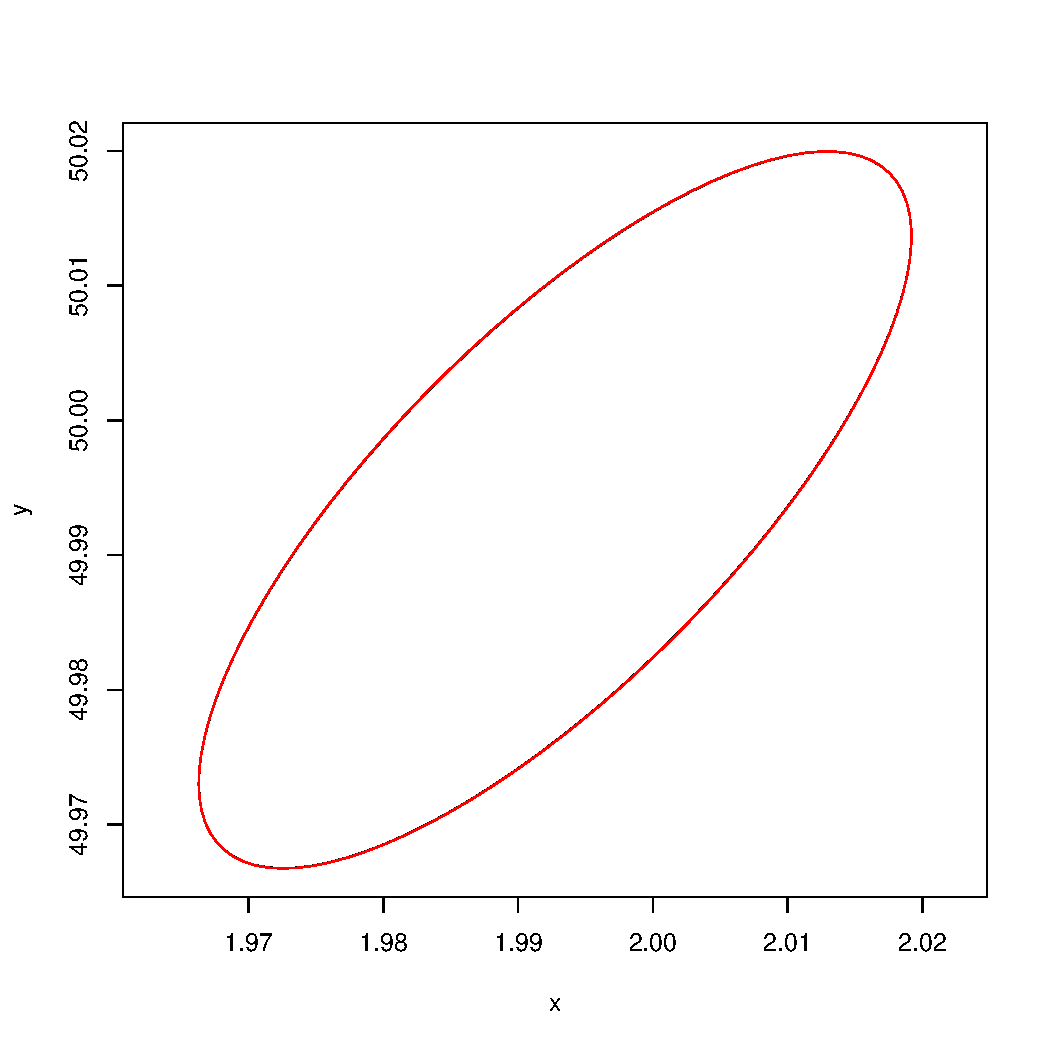
\includegraphics[width=\maxwidth,height=8cm]{figure/confRegion-1} 

\end{knitrout}

\begin{itemize}
	\item \texttt{which} should be a vector of size 2 that indicates the two components for which the confidence ellipse is to be constructed.

	\item \texttt{level} is the confidence level of the confidence region. The default is .95
\end{itemize}

\bigskip
\textbf{NOTE: }The argument  \texttt{confRegion} calls on the function \texttt{ellipse} in package \texttt{ellipse} to draw the ellipse.

\bigskip
\textbf{NOTE: } Since the confidence region is created for two parameters only, the size of the ellipse is determined by setting $p = 2$ irrespective of the original dimension of the problem.

\bigskip
To determine the effect of the confidence level, we draw two regions with difference confidence levels. We use \texttt{mcse.initseq} this time.

\begin{knitrout}
\definecolor{shadecolor}{rgb}{0.969, 0.969, 0.969}\color{fgcolor}\begin{kframe}
\begin{alltt}
\hlkwd{plot}\hlstd{(}\hlkwd{confRegion}\hlstd{(mcerror_is,} \hlkwc{which} \hlstd{=} \hlkwd{c}\hlstd{(}\hlnum{1}\hlstd{,}\hlnum{2}\hlstd{),} \hlkwc{level} \hlstd{=} \hlnum{.95}\hlstd{),} \hlkwc{type} \hlstd{=} \hlstr{'l'}\hlstd{,} \hlkwc{asp} \hlstd{=} \hlnum{1}\hlstd{)}
\hlkwd{lines}\hlstd{(}\hlkwd{confRegion}\hlstd{(mcerror_is,} \hlkwc{which} \hlstd{=} \hlkwd{c}\hlstd{(}\hlnum{1}\hlstd{,}\hlnum{2}\hlstd{),} \hlkwc{level} \hlstd{=} \hlnum{.90}\hlstd{),} \hlkwc{col} \hlstd{=} \hlstr{"red"}\hlstd{)}
\end{alltt}
\end{kframe}
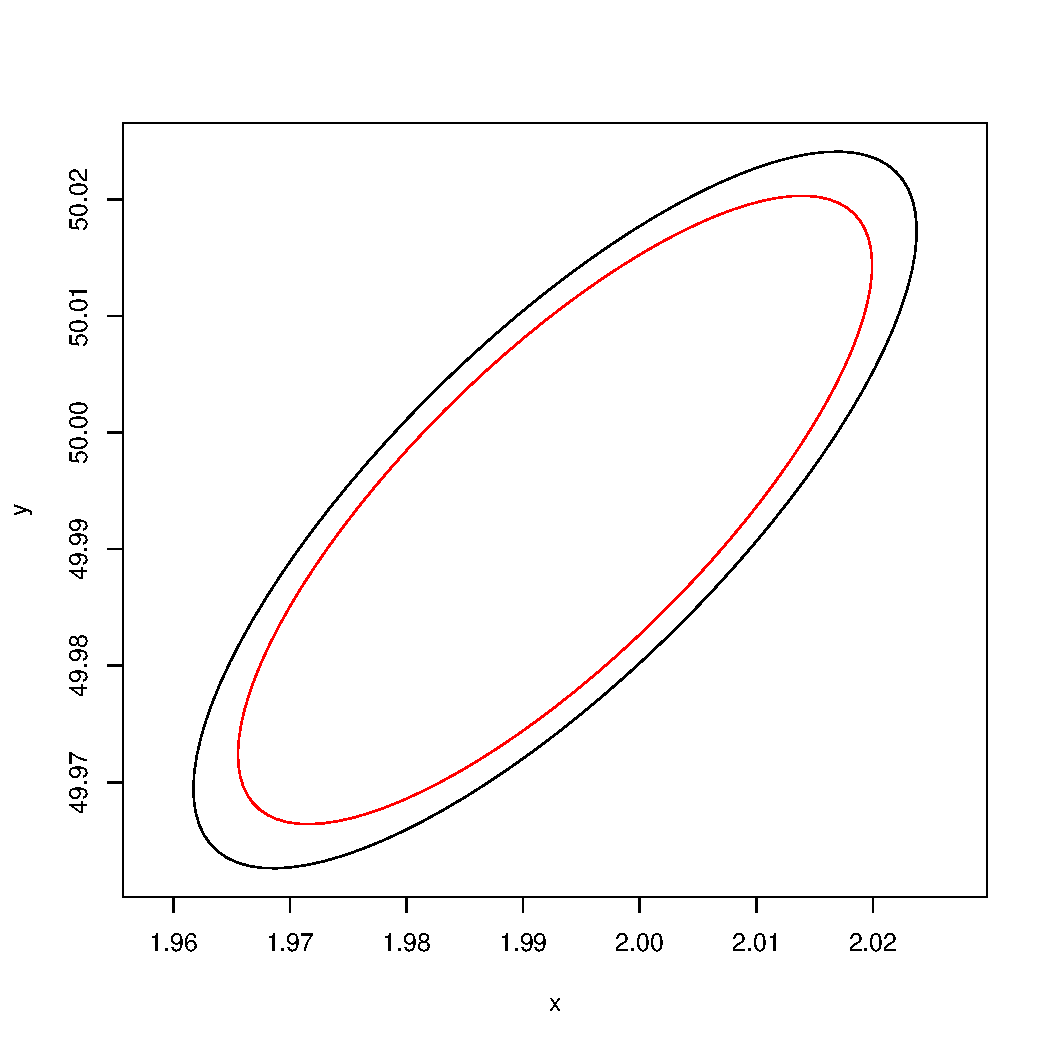
\includegraphics[width=\maxwidth,height=8cm]{figure/comp_region-1} 

\end{knitrout}

\section{Effective Sample Size}
Reporting $p \times p$ covariance matrix estimates is impractical and uninterpretable. The motivation of estimating Monte Carlo standard error is to ensure that said error is small. This is essentially the idea behind estimating effective sample size and ensuring that the estimated effective sample size is larger than a prespecified lower bound.

Before sampling the Markov chain, the user is advised to used the function \texttt{minESS} to ascertain what is the minimum effective sample size needed for stable analysis. See \cite{vats:fleg:jones:2017b} for theoretical details.
\begin{knitrout}
\definecolor{shadecolor}{rgb}{0.969, 0.969, 0.969}\color{fgcolor}\begin{kframe}
\begin{alltt}
\hlcom{# For mu}
\hlkwd{minESS}\hlstd{(}\hlkwc{p} \hlstd{=} \hlnum{3}\hlstd{,} \hlkwc{alpha} \hlstd{=} \hlnum{.05}\hlstd{,} \hlkwc{eps} \hlstd{=} \hlnum{.05}\hlstd{)}
\end{alltt}
\begin{verbatim}
## minESS 
##   8123
\end{verbatim}
\begin{alltt}
\hlcom{#For mu_g}
\hlkwd{minESS}\hlstd{(}\hlkwc{p} \hlstd{=} \hlnum{1}\hlstd{,} \hlkwc{alpha} \hlstd{=} \hlnum{.05}\hlstd{,} \hlkwc{eps} \hlstd{=} \hlnum{.05}\hlstd{)}
\end{alltt}
\begin{verbatim}
## minESS 
##   6146
\end{verbatim}
\end{kframe}
\end{knitrout}

\begin{itemize}
	\item \texttt{p} is the dimension of the estimation problem.
	\item \texttt{alpha} is the confidence level
	\item \texttt{eps} is the tolerance level. Default is .05. Reasonable levels are anywhere from .01 to .05. The smaller the tolerance, the larger the minimum effective samples. \texttt{eps} represents a tolerance level relative to the variability in the target distribution. It is akin to the idea of margin-of-error.
\end{itemize}

\texttt{minESS} is independent of the Markov chain or process, and is only a function of the  $p$, $\alpha$, and $\epsilon$. The user should find \texttt{minESS} and then sample their process until the required minimum samples are achieved. 

Alternatively, we often don't have to luxury of obtaining a lot of samples, and reaching a minimum effective sample size os not possible. In such a scneario, it is useful to know the $\epsilon$ tolerance level the number of estimated effective samples correspond to. So if we can only obtain 1000 effective samples,
\begin{knitrout}
\definecolor{shadecolor}{rgb}{0.969, 0.969, 0.969}\color{fgcolor}\begin{kframe}
\begin{alltt}
\hlcom{# For mu}
\hlkwd{minESS}\hlstd{(}\hlkwc{p} \hlstd{=} \hlnum{3}\hlstd{,} \hlkwc{alpha} \hlstd{=} \hlnum{.05}\hlstd{,} \hlkwc{ess} \hlstd{=} \hlnum{1000}\hlstd{)}
\end{alltt}
\begin{verbatim}
##   Epsilon 
## 0.1425016
\end{verbatim}
\begin{alltt}
\hlcom{#For mu_g}
\hlkwd{minESS}\hlstd{(}\hlkwc{p} \hlstd{=} \hlnum{1}\hlstd{,} \hlkwc{alpha} \hlstd{=} \hlnum{.05}\hlstd{,} \hlkwc{ess} \hlstd{=} \hlnum{1000}\hlstd{)}
\end{alltt}
\begin{verbatim}
##  Epsilon 
## 0.123959
\end{verbatim}
\end{kframe}
\end{knitrout}

Thus, if you obtained a sample with estimates effective sample size equaling 1000 for estimating $\mu_g$ and $\mu_{n,g}$, then the precision level of your estimate is $\epsilon = .143$ and $\epsilon = .124$, respectively.
\texttt{multiESS} and \texttt{ess} are two functions that calculate the effective sample size of a correlated sample. \texttt{ess} calculations are based on \cite{gong2015practical} and is component-wise, and \texttt{multiESS} utilizes the multivariate nature of the problem.

%<<ess>>=
%ess(chain)
%@

Since \texttt{ess} produces a different estimate for each component, conservative practice dictates choosing the smallest of the values. \texttt{multiESS} returns one estimate of the effective sample size based on the whole sample. The function calls \texttt{mcse.multi} function to obtain a batch means estimate of $\Sigma$. The user can provide another estimate of $\Sigma$ using the \texttt{covmat} argument.

\begin{knitrout}
\definecolor{shadecolor}{rgb}{0.969, 0.969, 0.969}\color{fgcolor}\begin{kframe}
\begin{alltt}
\hlkwd{multiESS}\hlstd{(chain)}
\end{alltt}
\begin{verbatim}
## [1] 31630.92
\end{verbatim}
\begin{alltt}
\hlcom{# Using spectral variance estimators}
\hlkwd{multiESS}\hlstd{(chain,} \hlkwc{covmat} \hlstd{= mcerror_bart}\hlopt{$}\hlstd{cov)}
\end{alltt}
\begin{verbatim}
## [1] 31231.11
\end{verbatim}
\begin{alltt}
\hlcom{# Using initial sequence estimators}
\hlcom{# Since this is a conservative estimator, ess will be smaller}
\hlkwd{multiESS}\hlstd{(chain,} \hlkwc{covmat} \hlstd{= mcerror_is}\hlopt{$}\hlstd{cov)}
\end{alltt}
\begin{verbatim}
## [1] 30544.9
\end{verbatim}
\end{kframe}
\end{knitrout}

Since the effective sample size is less than the minimum effective samples, we should simulate more. Looking at the ratio of the Monte Carlo samples size of $10^4$ and multiESS, we might need around $28,000$ Monte Carlo samples. 

\begin{knitrout}
\definecolor{shadecolor}{rgb}{0.969, 0.969, 0.969}\color{fgcolor}\begin{kframe}
\begin{alltt}
\hlkwd{set.seed}\hlstd{(}\hlnum{100}\hlstd{)}
\hlstd{chain} \hlkwb{<-} \hlkwd{mAr.sim}\hlstd{(}\hlkwc{w} \hlstd{=} \hlkwd{rep}\hlstd{(}\hlnum{2}\hlstd{,p),} \hlkwc{A} \hlstd{= A,} \hlkwc{C} \hlstd{= C,} \hlkwc{N} \hlstd{=} \hlnum{28000}\hlstd{)}

\hlcom{# larger than 8123}
\hlkwd{multiESS}\hlstd{(chain)}
\end{alltt}
\begin{verbatim}
## [1] 8952.358
\end{verbatim}
\begin{alltt}
\hlcom{# larger than 8123}
\hlkwd{multiESS}\hlstd{(chain,} \hlkwc{covmat} \hlstd{= mcerror_bart}\hlopt{$}\hlstd{cov)}
\end{alltt}
\begin{verbatim}
## [1] 8769.534
\end{verbatim}
\begin{alltt}
\hlcom{# larger than 8123}
\hlkwd{multiESS}\hlstd{(chain,} \hlkwc{covmat} \hlstd{= mcerror_is}\hlopt{$}\hlstd{cov)}
\end{alltt}
\begin{verbatim}
## [1] 8576.849
\end{verbatim}
\end{kframe}
\end{knitrout}
So no matter which estimator we choose for the Monte Carlo standard error, 28000 Monte Carlo samples are sufficient to have $\epsilon = .05$ relative tolerance.

\textbf{NOTE:} Ideally, we do not want to get more samples using the last iteration of the previous Markov chain. However, \texttt{mAr.sim} does not allow user specified starting values, so to demonstrate the use of \texttt{minESS} and \texttt{multiESS}, we get a new sample altogether. When making \texttt{R} packages that simulate a Markov chain, it is often very useful to allow user specific starting values for this reason.


\section{Graphical Diagnostics}

The function \texttt{estvssamp} plots the Monte Carlo estimates versus the sample size for a component of the MCMC output. This plot indicates whether the Monte Carlo estimate has stabilized.

\begin{knitrout}
\definecolor{shadecolor}{rgb}{0.969, 0.969, 0.969}\color{fgcolor}\begin{kframe}
\begin{alltt}
\hlkwd{estvssamp}\hlstd{(chain[,}\hlnum{1}\hlstd{])}
\end{alltt}
\end{kframe}
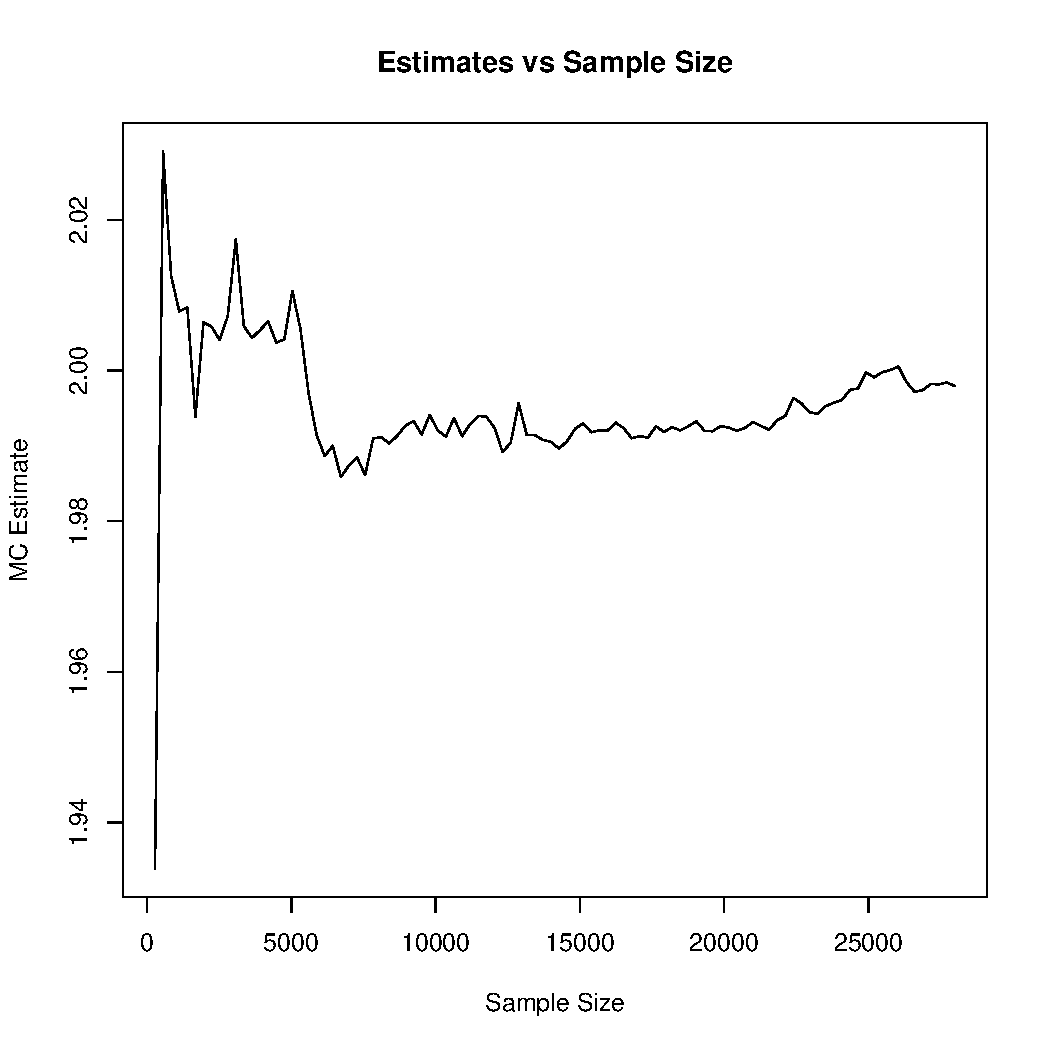
\includegraphics[width=8cm]{figure/estvssamp-1} 

\end{knitrout}

Additionally, if $p$ is not too small, due to the central limit theorem in \eqref{eq:clt} and an estimate of $\Sigma$ using the \texttt{mcse.multi} function, a QQ plot of the standardized estimates gives an idea of whether asymptopia has been achieved.

We generate a new Markov chain with $p = 50$.

\begin{knitrout}
\definecolor{shadecolor}{rgb}{0.969, 0.969, 0.969}\color{fgcolor}\begin{kframe}
\begin{alltt}
\hlstd{p} \hlkwb{<-} \hlnum{50}
\hlstd{A} \hlkwb{<-} \hlkwd{diag}\hlstd{(}\hlkwd{seq}\hlstd{(}\hlnum{.1}\hlstd{,} \hlnum{.9}\hlstd{,} \hlkwc{length} \hlstd{= p))}
\hlstd{C} \hlkwb{<-} \hlkwd{diag}\hlstd{(}\hlkwd{rep}\hlstd{(}\hlnum{2}\hlstd{, p))}

\hlkwd{set.seed}\hlstd{(}\hlnum{100}\hlstd{)}
\hlstd{chain} \hlkwb{<-} \hlkwd{mAr.sim}\hlstd{(}\hlkwc{w} \hlstd{=} \hlkwd{rep}\hlstd{(}\hlnum{2}\hlstd{,p),} \hlkwc{A} \hlstd{= A,} \hlkwc{C} \hlstd{= C,} \hlkwc{N} \hlstd{=} \hlnum{10000}\hlstd{)}
\end{alltt}
\end{kframe}
\end{knitrout}

For this new Markov chain, we find an estimate of $\Sigma$ to use for the \texttt{qqTest} function.

\begin{knitrout}
\definecolor{shadecolor}{rgb}{0.969, 0.969, 0.969}\color{fgcolor}\begin{kframe}
\begin{alltt}
\hlstd{mcerror_bm} \hlkwb{<-} \hlkwd{mcse.multi}\hlstd{(chain,} \hlkwc{method} \hlstd{=} \hlstr{"bm"}\hlstd{,} \hlkwc{blather} \hlstd{=} \hlnum{TRUE}\hlstd{)}
\hlstd{mcerror_isadj} \hlkwb{<-} \hlkwd{mcse.initseq}\hlstd{(chain,} \hlkwc{adjust} \hlstd{=} \hlnum{TRUE}\hlstd{,} \hlkwc{blather} \hlstd{=} \hlnum{TRUE}\hlstd{)}
\hlkwd{qqTest}\hlstd{(mcerror_bm)}
\end{alltt}
\end{kframe}
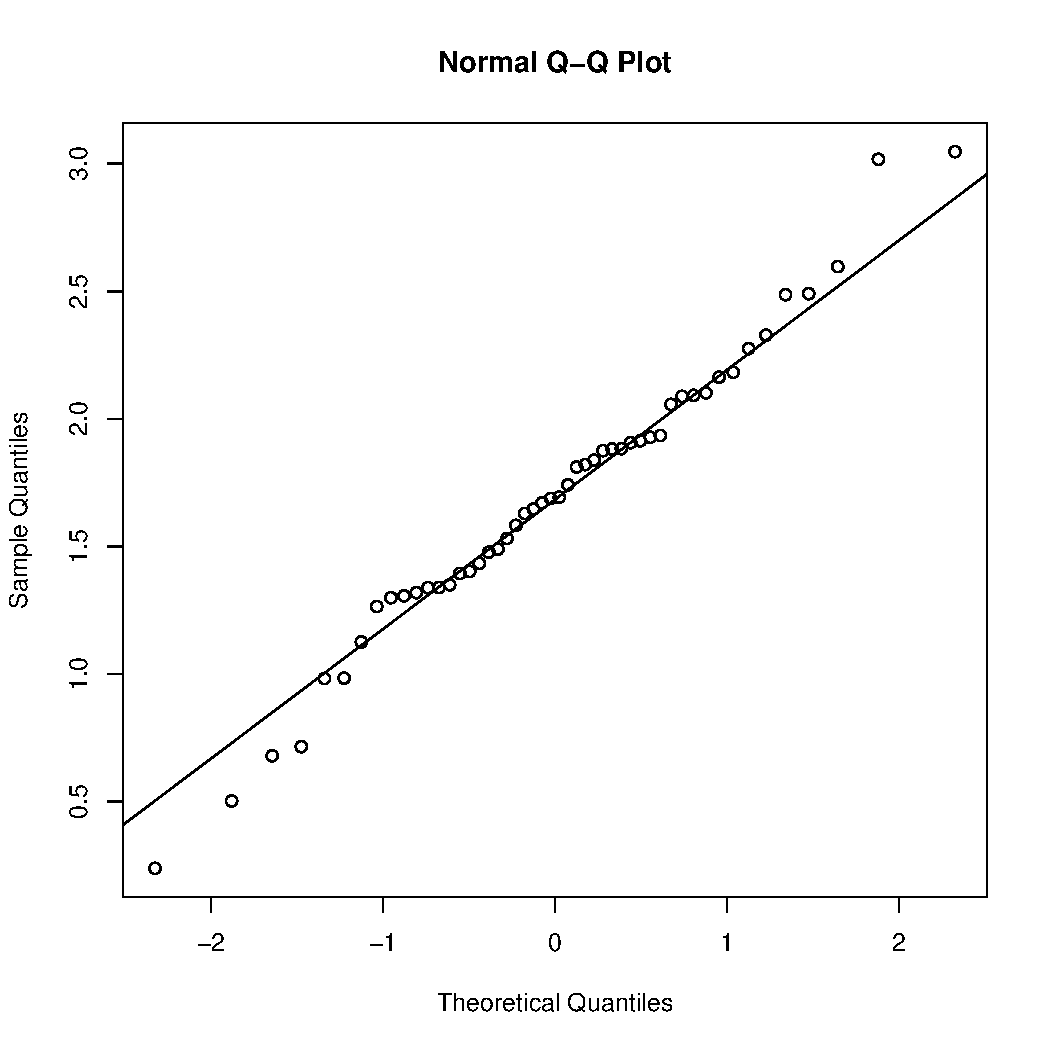
\includegraphics[width=8cm]{figure/qq-1} 
\begin{kframe}\begin{alltt}
\hlkwd{qqTest}\hlstd{(mcerror_isadj)}
\end{alltt}
\end{kframe}
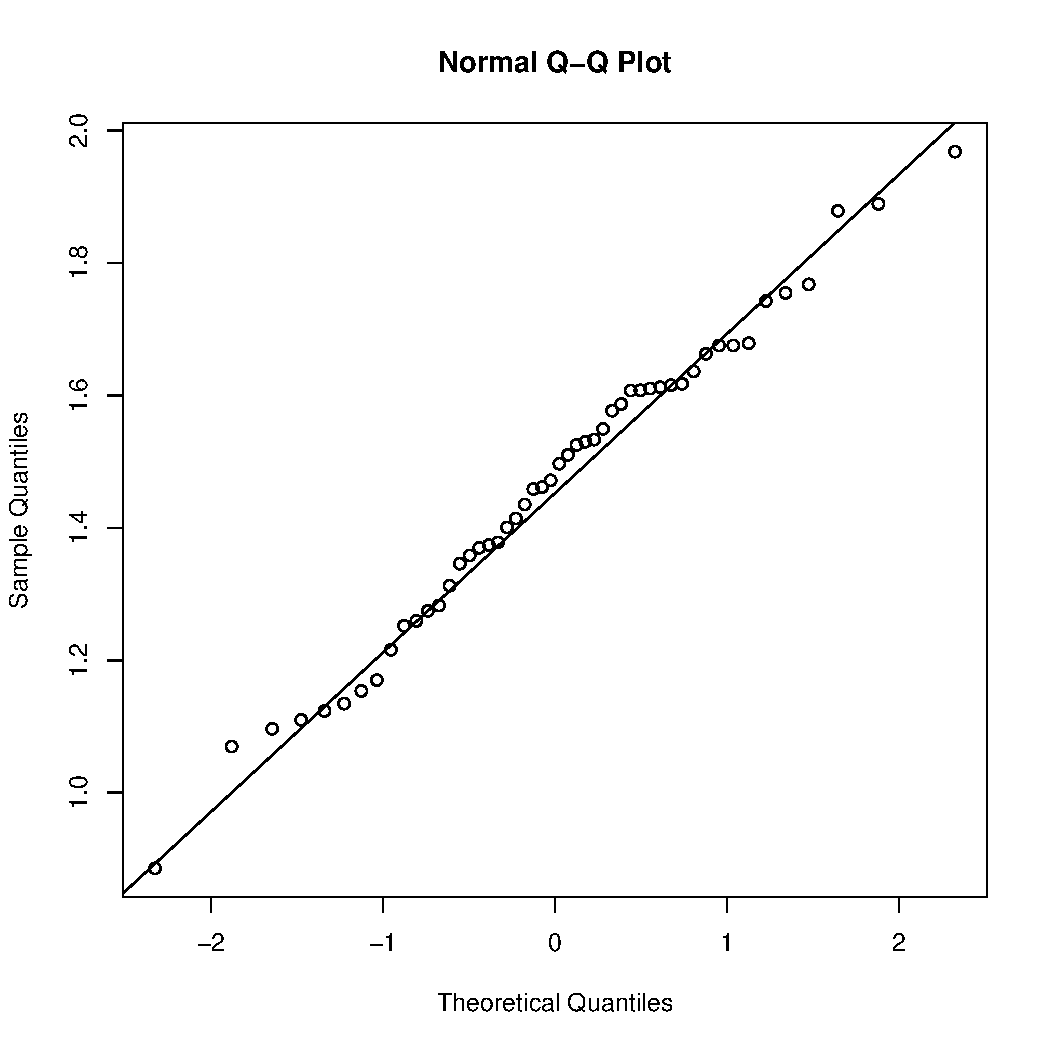
\includegraphics[width=8cm]{figure/qq-2} 

\end{knitrout}

Thus, we see here that the chain has not quite reached asymptopia.
\bibliographystyle{apalike}
\bibliography{mcse}

\end{document}
